%%%%%%%%%%%%%%%%%%%%%%%%%%%%%%%%%%%%%%%%%
% a0poster Landscape Poster
% LaTeX Template
% Version 1.0 (22/06/13)
%
% The a0poster class was created by:
% Gerlinde Kettl and Matthias Weiser (tex@kettl.de)
% 
% This template has been downloaded from:
% http://www.LaTeXTemplates.com
%
% License:
% CC BY-NC-SA 3.0 (http://creativecommons.org/licenses/by-nc-sa/3.0/)
%
%%%%%%%%%%%%%%%%%%%%%%%%%%%%%%%%%%%%%%%%%

%----------------------------------------------------------------------------------------
%	PACKAGES AND OTHER DOCUMENT CONFIGURATIONS
%----------------------------------------------------------------------------------------

\documentclass[a0,landscape]{a0poster}

\usepackage{multicol} % This is so we can have multiple columns of text side-by-side
\columnsep=90pt % This is the amount of white space between the columns in the poster
\columnseprule=3pt % This is the thickness of the black line between the columns in the poster

\usepackage[svgnames]{xcolor} % Specify colors by their 'svgnames', for a full list of all colors available see here: http://www.latextemplates.com/svgnames-colors

\usepackage{times} % Use the times font
%\usepackage{palatino} % Uncomment to use the Palatino font
\usepackage{float} % Allows putting an [H] in \begin{figure} to specify the exact location of the figure
\usepackage{graphicx} % Required for including images
\graphicspath{{figures/}} % Location of the graphics files
\usepackage{booktabs} % Top and bottom rules for table
\usepackage[font=small,labelfont=bf]{caption} % Required for specifying captions to tables and figures
\usepackage{amsfonts, amsmath, amsthm, amssymb} % For math fonts, symbols and environments
\usepackage{wrapfig} % Allows wrapping text around tables and figures
\usepackage[center]{titlesec}
\usepackage{background}
\usepackage{blindtext}
\usepackage{euler}
\backgroundsetup{
scale=1,
angle=0,
opacity=1,
contents={\begin{tikzpicture}[remember picture,overlay] 
\path [bottom color = Maroon!20!white, top color = white] (current page.south west)rectangle (current page.north east);\end{tikzpicture}}
}
\begin{document}

%----------------------------------------------------------------------------------------
%	POSTER HEADER 
%----------------------------------------------------------------------------------------

% The header is divided into three boxes:
% The first is 55% wide and houses the title, subtitle, names and university/organization
% The second is 25% wide and houses contact information
% The third is 19% wide and houses a logo for your university/organization or a photo of you
% The widths of these boxes can be easily edited to accommodate your content as you see fit

\begin{minipage}[b]{0.5\textwidth}
\veryHuge \color{Brown} \textbf{Radio Cosmology Lab} \color{Black}\textbf{$|$} \color{Black}\LARGE\textit{Exploring the Epoch of Reionization}\\
\textbf{Adam Lanman, Wenyang Li, Joshua Kerrigan,\\ Jacob Burba, Peter Sims, Jonathan Pober}\\ % Author(s)
\huge Brown University Physics\\ % University/organization
\end{minipage}
\begin{minipage}[b]{0.6\linewidth}

\includegraphics[width=45cm]{radiologo_update.png} % Logo or a photo of you, adjust its dimensions here
\end{minipage}
%I CANT SEEM TO GET THIS DAMN LOGO TO THE RIGHT

%[Maybe put logos at the top(or bottom), PAPER doesn't have an official logo afaik, can't find a good one for MWA]
%\hspace{5cm}
%\begin{minipage}[b]{0.15\linewidth}
%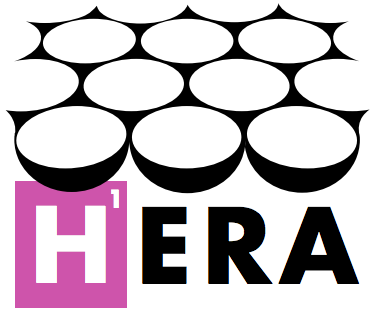
\includegraphics[width=15cm]{HERA.png} % Logo or a photo of you, adjust its dimensions here
%\end{minipage}
%\hspace{2cm}
%\begin{minipage}[b]{0.15\linewidth}
%\Huge{\textbf{PAPER}}
%\end{minipage}
%\hspace{2cm}
%\begin{minipage}[b]{0.15\linewidth}
%\Huge{\textbf{MWA}}
%\end{minipage}

%
%\begin{minipage}[b]{0.25\linewidth}
%\color{DarkSlateGray}\Large \textbf{Contact Information:}\\
%Physics\\ % Address
%Brown University\\
%$\#$ George St., Providence, RI\\\\
%Phone: +1 (000) 111 1111\\ % Phone number
%Email: \texttt{Add Emails}\\ % Email address
%\end{minipage}
%
% Maybe we don't need the Brown logo, consider replacing with PAPER,HERA,MWA logos?


%\vspace{1cm} % A bit of extra whitespace between the header and poster content

%----------------------------------------------------------------------------------------

\begin{multicols}{4} % This is how many columns your poster will be broken into, a poster with many figures may benefit from less columns whereas a text-heavy poster benefits from more

%----------------------------------------------------------------------------------------
%	ABSTRACT
%----------------------------------------------------------------------------------------

%\color{Navy} % Navy color for the abstract

%\begin{abstract}

%Following the recombination of hydrogen and release of the cosmic microwave background radiation at redshift $z \sim 1100$, the baryonic matter of the universe consisted mostly of neutral hydrogen and helium. Gradually, small inhomogeneities collapsed and ignited the first luminous structures. Energetic photons emitted from the first stars and quasars reionized the surrounding medium, producing ionized bubbles which grew and merged into the fully ionized intergalactic medium we see today. This \emph{Epoch of Reionization} (EoR) remains a poorly-understood period of the universe's history which offers a wealth of cosmological and astrophysical information.

%The Pober lab is part of an international effort to build instruments capable of studying the EoR. The neutral hydrogen (HI) of the EoR emits faintly at a wavelength of 21cm, due to the hyperfine transition. This emission is unique to neutral hydrogen, and is anti-correlated with the ionized (HII) regions that fill the universe through the EoR. CMB constraints and quasar absorption spectra put the EoR as occurring within the redshift range $6 < z < 12$, which means 21cm emissions will redshift to meter scale wavelengths. This is accessible to modern radio interferometers, including the \emph{Donald C. Backer Precision Array for Probing the Epoch of Reionization} (PAPER), the \emph{Murchison Widefield Array} (MWA), and the recently-funded \emph{Hydrogen Epoch of Reionization Array} (HERA).

%The main focus of the Pober Lab is the direct observation of the 21cm Neutral Hydrogen (HI) emission through the use of radio telescope arrays to detect the signal from the Epoch of Reionization (EoR). The 21cm hyperfine spin flip, which is typically a forbidden transition, has a mean lifetime on the order of 100 million years. This time scale, and the abundance of HI in the universe gives us the ability to map the progress of reionization which has the redshift range of 6 $<$ z $<$ 12. To observe the reionization of the HI, we use radio telescope arrays, because the 21cm emission corresponds to 1420 MHz at rest and when received at Earth corresponds to 100-200 MHz due to cosmological redshifting. The Pober Lab contributes to several international radio telescope array collaborations which include the Precision Array for Probing the Epoch of Reionization (PAPER), the Murchison Widefield Array (MWA) and the newly NSF funded Hydrogen Epoch of Reionization Array (HERA).

%\end{abstract}

%----------------------------------------------------------------------------------------
%	INTRODUCTION
%----------------------------------------------------------------------------------------
\color{DarkSlateGray}  % SaddleBrown color for the introduction

\section*{Introduction}
Following the recombination of hydrogen and release of the cosmic microwave background radiation, the baryonic matter of the universe consisted mostly of neutral hydrogen and helium. Gradually, small inhomogeneities collapsed and ignited into the first luminous structures. Energetic photons emitted from the first stars and quasars reionized the surrounding medium, producing ionized bubbles which grew and merged into the fully ionized intergalactic medium we see today. This \emph{Epoch of Reionization} (EoR) remains a poorly-understood period of the universe's history which offers a wealth of cosmological and astrophysical information.

The Pober lab is part of an international effort to build instruments capable of studying the EoR. The neutral hydrogen (HI) of the EoR emits faintly at a wavelength of 21cm due to the hyperfine transition. This emission is unique to neutral hydrogen, and is anti-correlated with the ionized (HII) regions that fill the universe through the EoR. CMB constraints and quasar absorption spectra place the EoR within the redshift range $6 < z < 12$, which means 21cm emissions will reach us at meter scale wavelengths. This is accessible to modern radio interferometers, including the \emph{Donald C. Backer Precision Array for Probing the Epoch of Reionization} (PAPER), the \emph{Murchison Widefield Array} (MWA), and our newly observing \emph{Hydrogen Epoch of Reionization Array} (HERA). Extracting this weak signal remains a challenge unprecedented in radio astronomy.



\subsubsection*{Differential Brightness Temperature}
%\begin{equation}
%\label{difftemp}
%\resizebox{.9\hsize}{!}{$
%\delta T_{b} = 28mK(1+\delta)x_{HI}\Big(1-\frac{T_{CMB}}{T_{spin}}\Big)\Big(\frac{\Omega_{b}h^2}{0.0223}\Big)%\sqrt{\Big(\frac{1+z}{10}\Big)\Big(\frac{0.24}{\Omega_m}\Big)}\Big[ \frac{H(z)/(1+z)}{dv_{||}/dr_{||}}\Big]$}%
%\end{equation}


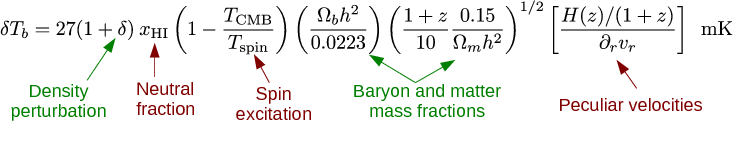
\includegraphics[scale=1]{figures/differential_brightness.png}
The differential brightness temperature $\delta T_b$ is the contrast between the intensity of 21 cm emissions/absorptions against the Cosmic Microwave Background. Its full expression is related to cosmological (green) and astrophysical (red) parameters. Figure \ref{global} shows the evolution of the spherically-averaged \emph{global} 21 cm brightness temperature.

\begin{figure}[H]
\centering
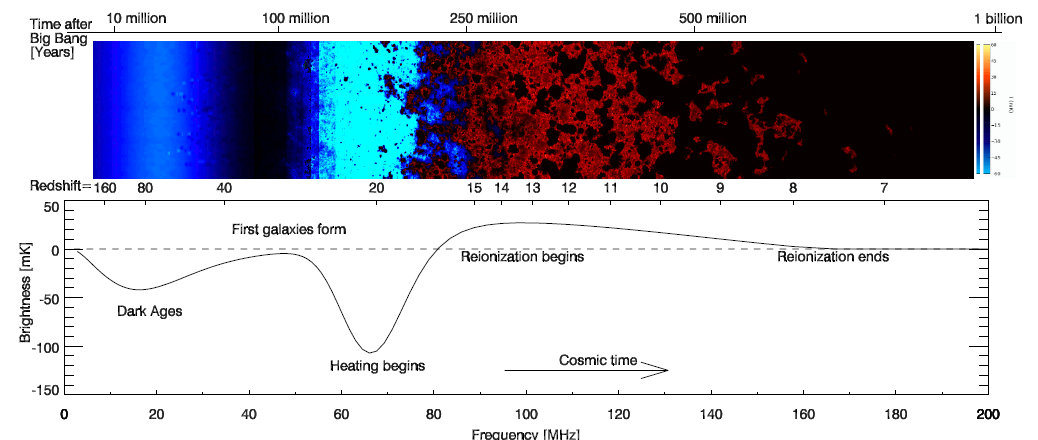
\includegraphics[width=1.0\linewidth]{figures/global_history.png}
\caption{The global differential brightness temperature, $\delta T_b$, evolution over redshift $6<z<160$. $\delta T_b$ becomes observable when the spin temperature $T_S$ decouples from the CMB temperature, $T_{CMB}$.
Eqn. \ref{difftemp}. Source: Pritchard \& Loeb. Nature 468.7325 (2010): 772-773. }\label{global}
\end{figure}

%----------------------------------------------------------------------------------------
%	OBJECTIVES
%----------------------------------------------------------------------------------------
% DarkSlateGray color for the rest of the content
\section*{The Foreground Problem} %[I dont need all of these plots, they're just there to be cut as needed or if necessary to take up more space]
%Galactic and extragalactic foregrounds pose a difficult problem when trying to measure the 21cm EoR signal. Relative to galactic foregrounds, the EoR signal is $\sim$ 5 orders of magnitude smaller than the galactic emissions that exist between our observing radio telescope arrays and the highly redshifted 21cm signal. The overlapping sources of power in our observations can be seen in Fig. \ref{fig:foregroundsrcs}.  -- Just making this shorter, and clarifying a bit on what the foregrounds are.

The expected EoR signal is $\sim$ 5 orders of magnitude weaker than known foreground sources, such as diffuse emission from the Galaxy and extragalactic point sources. Removing these foregrounds, as well as instrumental noise, is a nontrivial problem. An example of the overlapping sources of power in our observations can be seen in Fig. \ref{fig:foregroundsrcs}.


\begin{figure}[H]
\centering
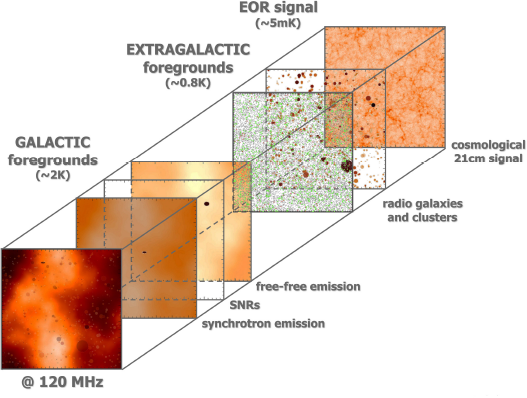
\includegraphics[width=0.55\linewidth]{figures/foreground_figure.png}
\caption{The various cosmological and galactic sources that contribute to the measured sky temperature, and their relative strengths.\\\hspace{\textwidth}
Source: Zaroubi, Saleem. \textit`{The First Galaxies}. Springer Berlin Heidelberg, 2013. 45-101.}\label{fig:foregroundsrcs}
\end{figure}
To overcome foreground dominance in our power spectrum analysis we can use a combination of foreground power mitigating techniques as outlined in the following subsections.
%The issue of foreground emission dominance in our power spectrum can be overcome through the mixed use of the following traditional and novel foreground mitigation techniques. \\
%\subsubsection*{Foreground Subtraction}
%Foreground subtraction is performed in the image domain using an extragalactic source catalog. The source catalog is used to generate a foreground model which can then be fit by an $n^{th}$ order polynomial and subtracted from the observation.
%Baseline visibilities are gridded to form an image which is calibrated to a catalog model. The catalog model contains point sources from 
%surveys which contain the sources' right ascension, declination, and flux in stokes I. The model built from the catalog of sources is 
%additionally convolved with the telescope arrays synthesized beam model. The resulting model which has been built can then be subtracted 
%from the observation leaving behind the EoR signal and diffuse emissions.

\subsubsection*{Hydrid Foreground Removal and Avoidance}
The need for managing foregrounds in 21cm EoR experiments has led to two distinct techniques: Avoidance and Removal. Avoidance is the practice of filtering out foregrounds in Fourier space. Removal requires an extragalactic point source catalog or Galactic diffuse emission models, that can be precisely subtracted from observations. The hybrid approach attempts to use both techniques to further mitigate foreground contamination for the purpose of an EoR detection in the 21cm power spectrum.

\begin{figure}[H]
\centering
\frame{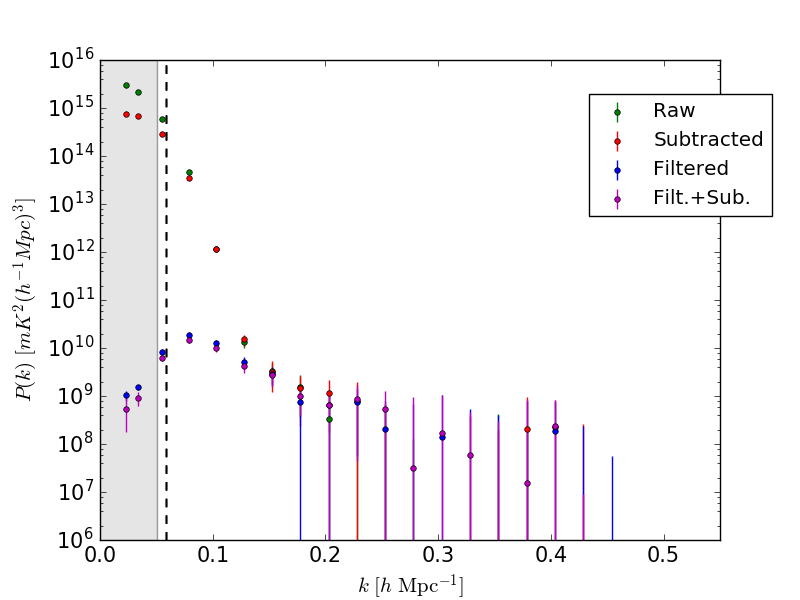
\includegraphics[width=0.6\linewidth]{figures/PSPECXMid.png}}
\caption{Power spectrum demonstrating the effectiveness of filtering, subtraction, and hybrid strategies for foreground removal and avoidance.}
\label{fig:stages}
\end{figure}

\begin{figure}[H]
\centering
\frame{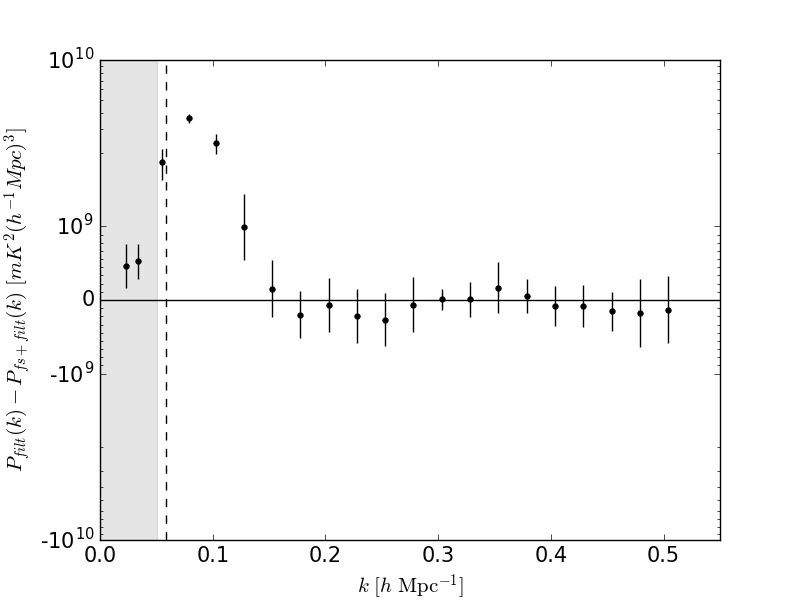
\includegraphics[width=0.6\linewidth]{figures/DIFFXMid.png}}
\caption{The difference power spectrum of Fig. \ref{fig:stages} demonstrating that the hybrid foreground removal and avoidance technique is able to remove 
additional foreground contamination necessary for placing the tightest constraints on the EoR power spectrum.}
\label{fig:diffmid}
\end{figure}

%\subsubsection*{Foreground Avoidance}
%\begin{equation}
%\label{delaytransform}
%V_b(\tau) = \int dl dm d\nu A(l,m,\nu)I(l,m,\nu)e^{-2\pi i\nu(\tau_g -\tau)}
%\end{equation}
%Equation \ref{delaytransform} demonstrates the delay transform used to transform a visibility to delay space. By working in delay space it can be seen in both Figs. \ref{foregroundsrcs1} \& \ref{foregroundsrcs2} that power from foreground sources are confined within a delay limit known as the horizon limit. --- this seemed unclear, so I made it a little longe

%Equation \ref{delaytransform} demonstrates the \emph{delay transform}: A Fourier transform of frequency to its conjugate \emph{delay}. There is a natural limit in delay, set by the time it takes light from a source at the horizon to travel between the two antennas of a baseline. Power from foreground sources is confined within this \emph{horizon limit}, as shown by Figs. \ref{foregroundsrcs1} \& \ref{foregroundsrcs2}.

%Taking the Fourier transform of a baseline visibility over frequency with the geometric group delay offset (eqn. \ref{delaytransform}) results %in smooth spectrum foregrounds bunching up nearest to the delay of $\tau = 0$. This is because foreground sources have a maximal %geometric delay associated with a baseline length, $|\vec{b}|$, which is also known as the horizon limit. The EoR signal is unsmooth %spectrally, distinguishing it from foreground sources, and pushing it beyond the horizon limit imposed by the baseline length. Using this %information, delays below the horizon limit can be filtered giving significant foreground power removal.

%\begin{figure}[H]
%\centering
%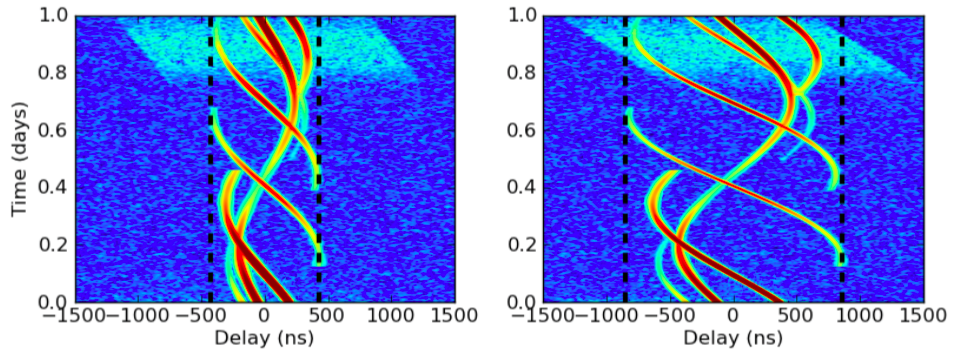
\includegraphics[width=0.8\linewidth]{figures/delaytransform.png}
%\caption{Delay transform visibilities of two different baseline types. Smooth spectral sources moving between delays over time can be seen to remain within the horizon limit (dotted), while unsmooth spectral sources (light blue) extend beyond the horizon limit.  \textbf{Source}: Aaron Parsons, \textit{A Per Baseline Delay-Spectrum Technique for Accessing the 21cm Cosmic Reionization Signature, Apj. 2012}}
%\label{foregroundsrcs2}
%\end{figure}

%----------------------------------------------------------------------------------------
%	MATERIALS AND METHODS
%----------------------------------------------------------------------------------------
\columnbreak
\section*{Simulation}

The particular characteristics of an array can introduce unexpected effects into the data. Understanding and mitigating instrumental effects is critical to making a confident detection of the EoR. For this reason, much effort has been put into simulating the full analysis pipeline -- from the point and diffuse sources on the sky, to the raw visibilities that come out of the correlator, to the power spectrum estimations.

Fast Holographic Deconvolution (FHD) is a purpose-built software framework for analyzing MWA data. FHD does foreground subtraction by \emph{forward modeling}, which builds a simulated data set, including instrumental effects, and subtracts it from the actual data. This forward modeling feature can also be used as a standalone simulation tool, to generate raw visibilities of foregrounds, noise, and EoR off of existing and future 21cm experiments.

\begin{figure}[H]
\centering
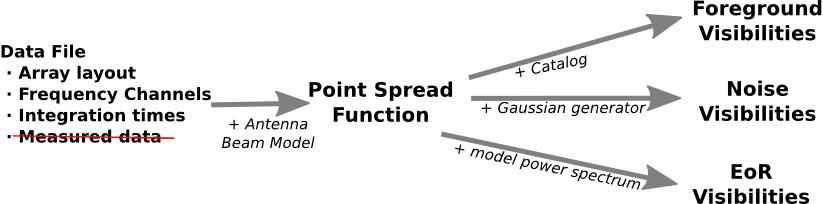
\includegraphics[scale=.9]{figures/sim_flowchart.png}
\caption{A sample data file (or generated data file) holds array coordinates over time and the frequency channels of the instrument. Given a beam model for the antenna, FHD calculates the full synthesized beam (or point-spread function) for a particular time and set of frequencies. The synthesized beam can then convert a sky catalog into a set of foreground visibilities for the instrument. External EoR simulations can also be fed in to test EoR sensitivity, or Gaussian noise can be injected to simulate noise.}
\end{figure}

%------------------------------------------------
\section*{Calibration}

%The most common techniques we use on visibility calibration are redundant calibration and sky model based calibration. Sky model calibration requires some preknowledge about the sky. With our assumptions about source structures of the sky and understanding of our instrument, we use FHD (Fast Holographic Deconvolution) to calibrate visibility data. The algorithm FHD uses is basically 'CLEAN' algorithm. Redundant calibration is sky model independent. All it assumes is that same antenna separations should measure exact the same Fourier mode of the sky. Redundant calibration requires antenna array with good redundant calibratability, like PAPER64, MWA PhaseII hexes and HERA.  -- [I cut the (Fast Holographic Deconvolution) since I gave the acronym earlier.]

21~cm observations of the Epoch of Reionization (EoR) have the potential to reveal a wealth of information about the formation of the first stars and galaxies by measuring the three dimensional power spectrum and full tomographic maps of the neutral IGM. However, these observations are technically very challenging due to bright astrophysical foregrounds and the chromatic nature of radio interferometers. In the last two years it has become apparent that precision instrument calibration is crucial for disentangling the faint cosmological signal from the bright foregrounds. Current precision calibration efforts for EoR observations fall into two camps:  sky based calibration using deep foreground catalogs and forward modelling of the instrument visibilities, and redundant calibration that foregoes a sky model but requires the tiles be placed on a precise grid.
\begin{figure}[H]
\centering
\label{comparison_between_FHD_and_OMNICAL}
\frame{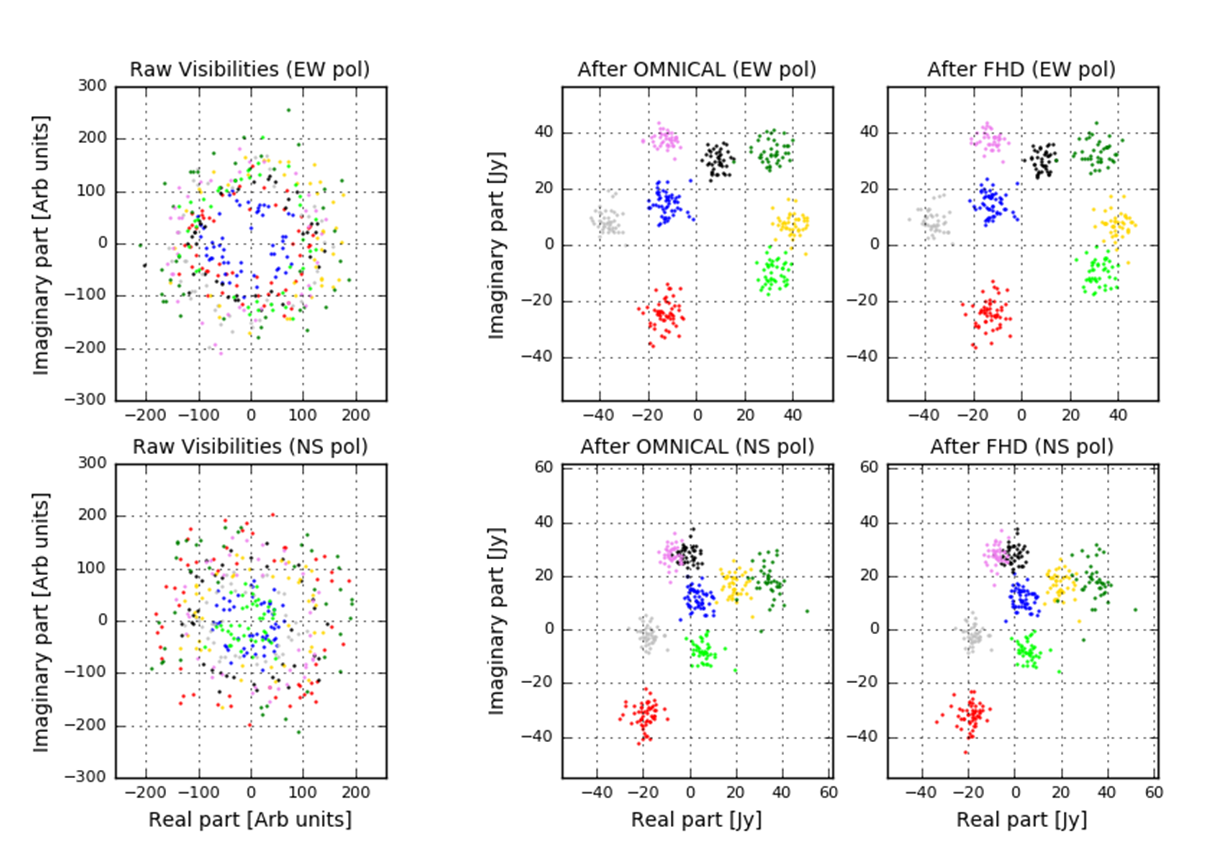
\includegraphics[width=1.0\linewidth]{figures/f299.png}}
\caption{2 min averaged complex visibilities of EoR0 observation by MWA II at 191MHz from 8 redundant baseline groups. Each color represents one baseline group. Left column: raw visibilities, with arbitrary units; Middle column: visibilities after \texttt{OMNICAL}, with degeneracy parameters projected (units: Jy); Right column: visibilities after FHD sky calibration (units: Jy). Top row: East-West polarization; Bottom row: North-South polarization.}
\end{figure}


%----------------------------------------------------------------------------------------
%	RESULTS 
%----------------------------------------------------------------------------------------

\section*{Hydrogen Epoch of Reionization Array (HERA)}
%\begin{figure}[H]
%\centering
%\label{fig:PAPER}
%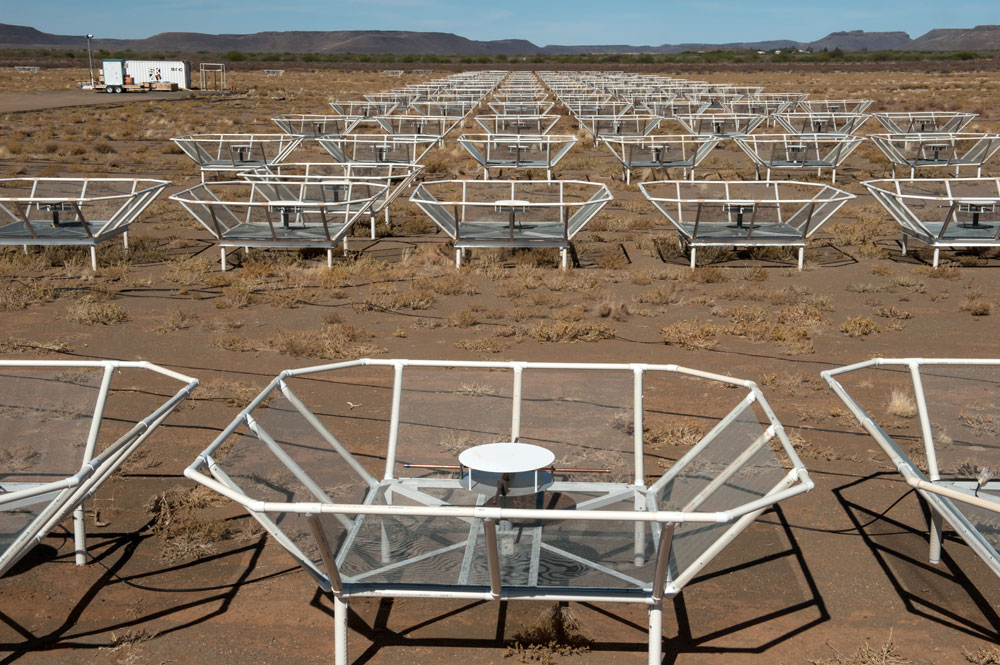
\includegraphics[width=0.85\linewidth]{figures/paper}
%\caption{PAPER - A first-generation array located in the Karoo desert of South Africa. Designed specifically for EoR research, PAPER is designed for maximum redundancy. Several baselines sample each $k_\perp$ modes, which allows for the use of redundant calibration.}
%\end{figure}

%\begin{figure}[H]
%\centering
%\label{fig:MWA}
%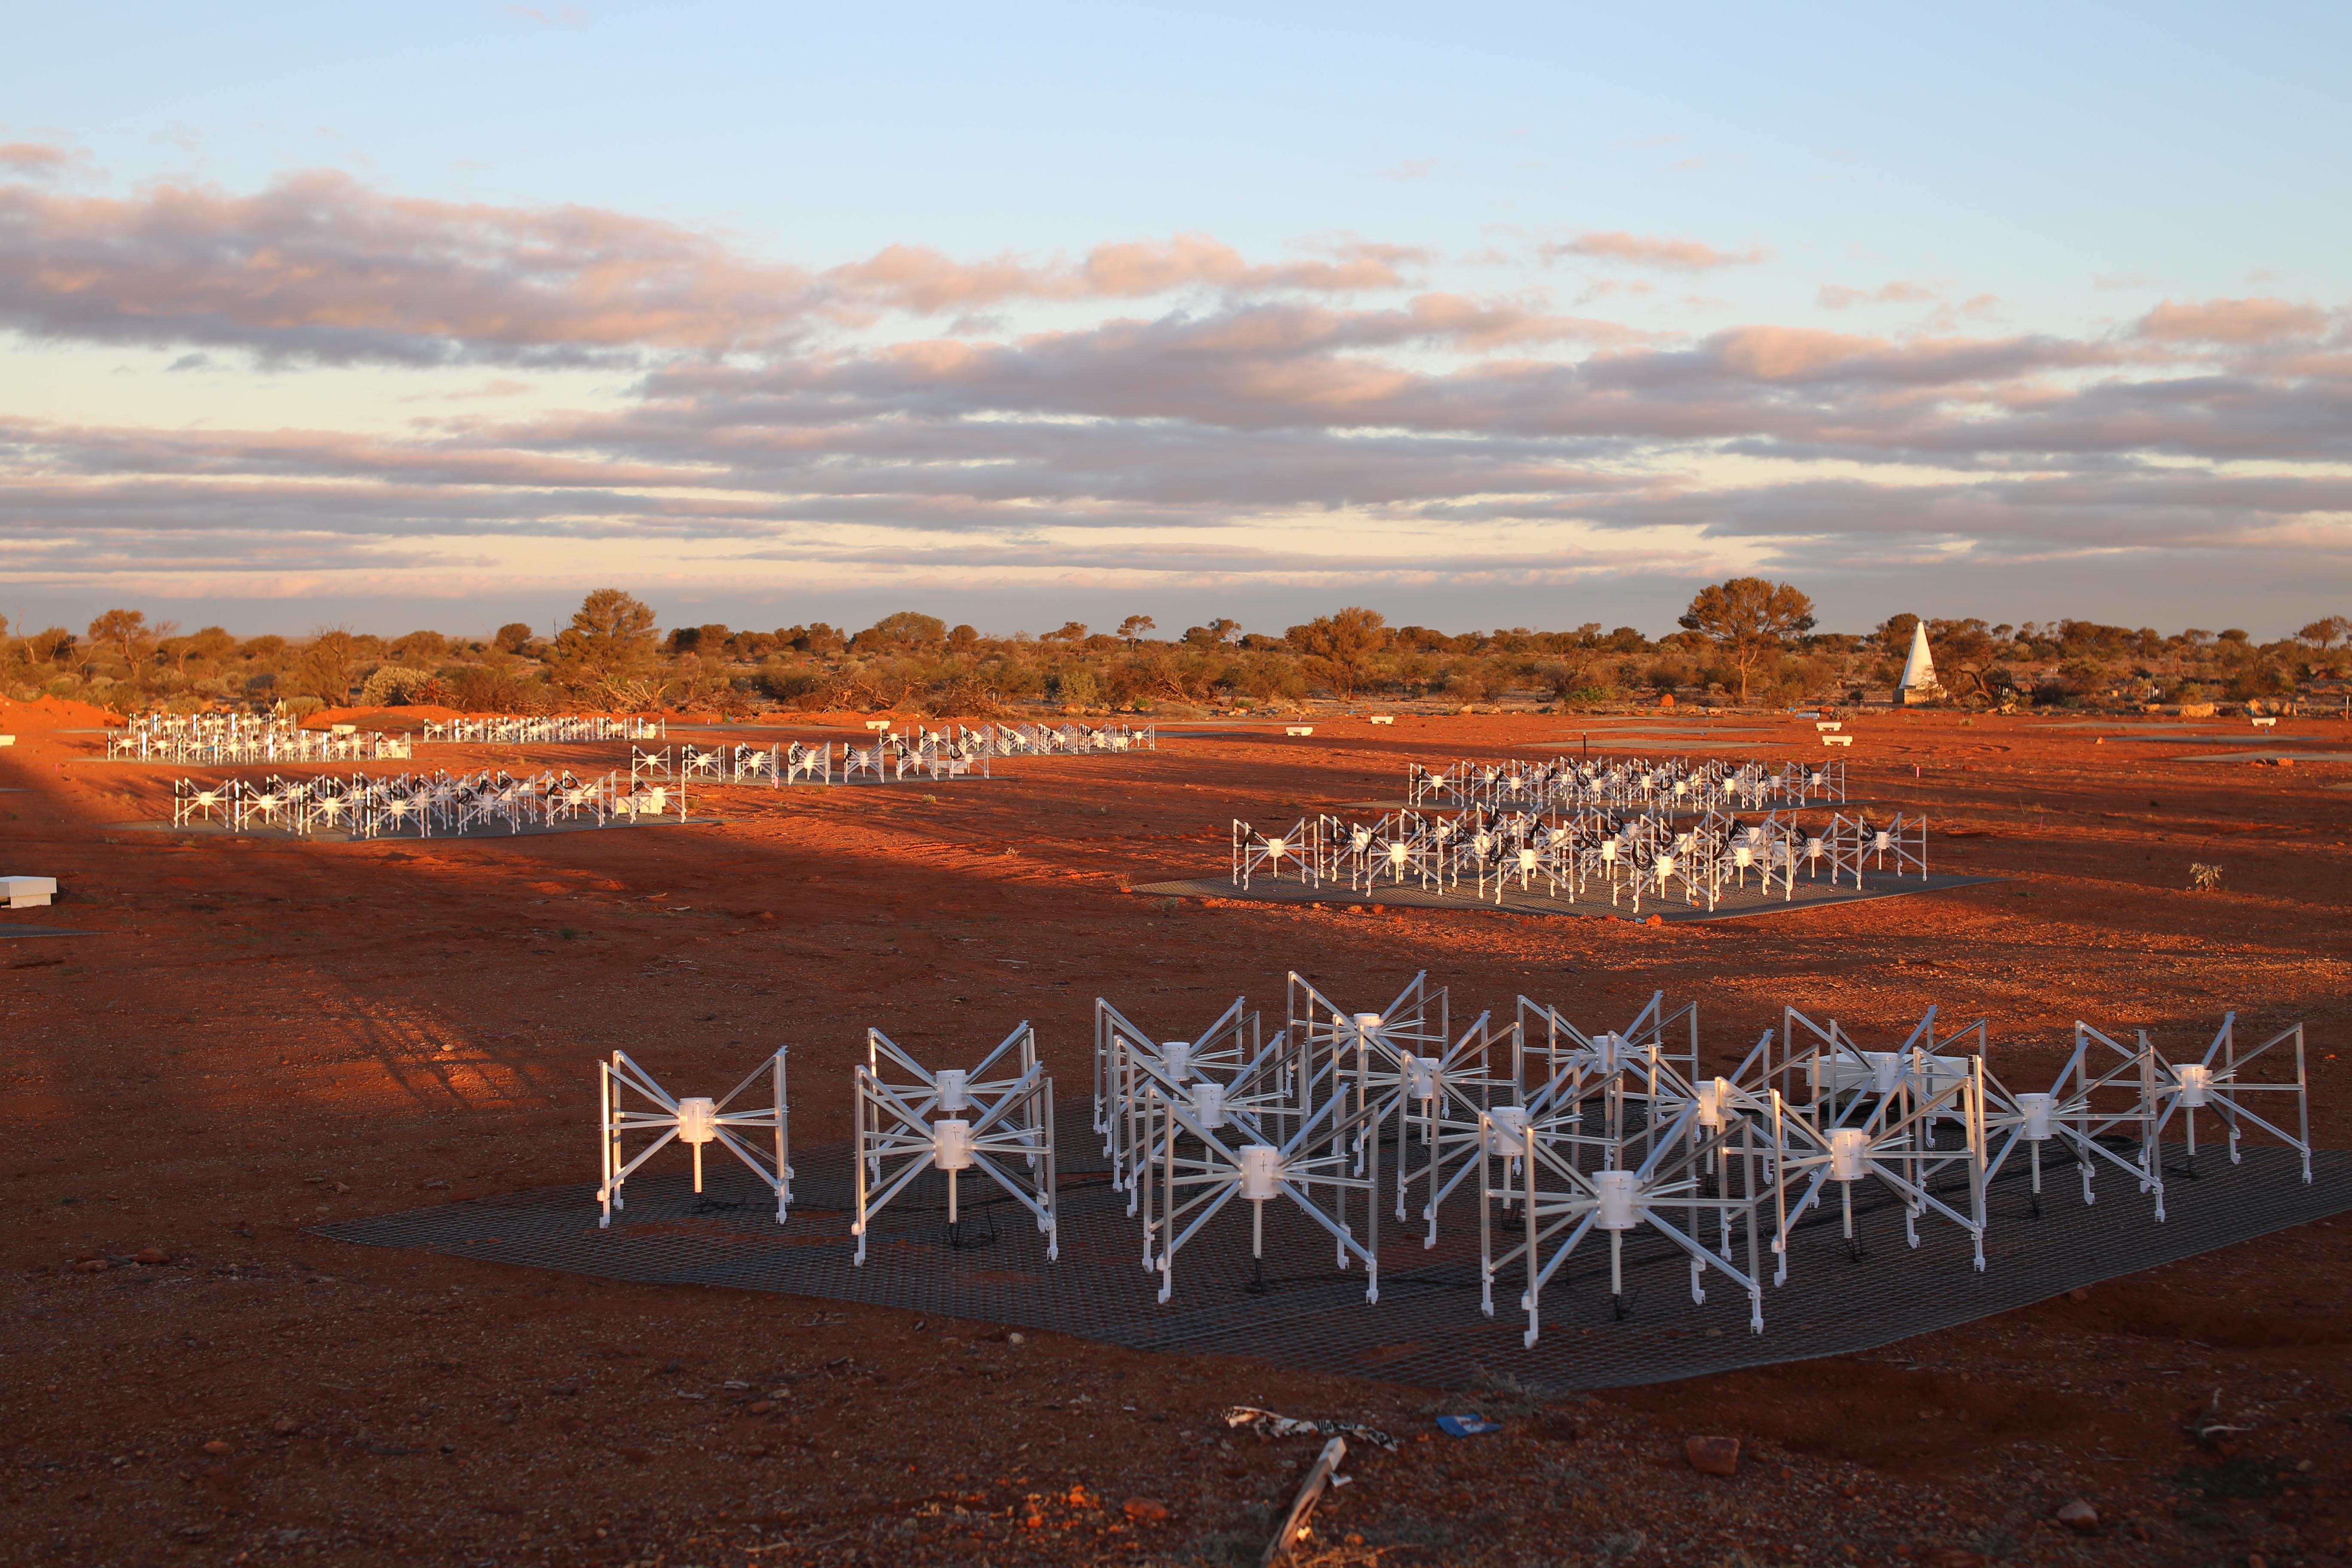
\includegraphics[width=0.85\linewidth]{figures/phaseII_tiles.jpg}
%\caption{MWA - Located in Western Australia at the Murchison Radio Astronomy Observatory. The MWA serves multiple functions, including ionosphere studies and detection of transient radio signals. Phase I consisted of 128 tiles which are each made up of 16 dipole antennae. The Phase I configuration maximized uv coverage, improving imaging capability. It has since been partially reconfigured into Phase II, which includes two hexagonal grids of tiles designed for high-redundancy EoR research. MWA is a pathfinder project for the Square Kilometer Array (SKA).}
%\end{figure}
The Hydrogen Epoch of Reionization Array is the next generation telescope observing the 21 cm emission from neutral intergalactic medium (IGM) during the epoch of reionization (z = 6 - 12), and a precursor instrument for Square Kilometer Array (SKA). The HERA instrument will be an interferometer with 350 14-meter parabolic dishes in South Africa. These elements will be divided into 320-element hexagonal shaped core and 30 outriggers. The current stage of HERA has 37 dishes deployed. 

Although increasingly stringent upper limits of 21 cm signal has been placed by the first generation experiments targeting EoR such as Precision Array for Probing the Epoch of Reionization array (PAPER), Murchison Widefield Array (MWA) and LOw Frequency ARray (LOFAR), they are not able to detect it due to their sensitivity limits. HERA is designed to bring both the sensitivity and the precision to directly constrain the topology and evolution of reionization. This will push forward our understanding of the formation of first stars and galaxies. \\

\begin{figure}[H]
\centering
\label{fig:HERA}
\frame{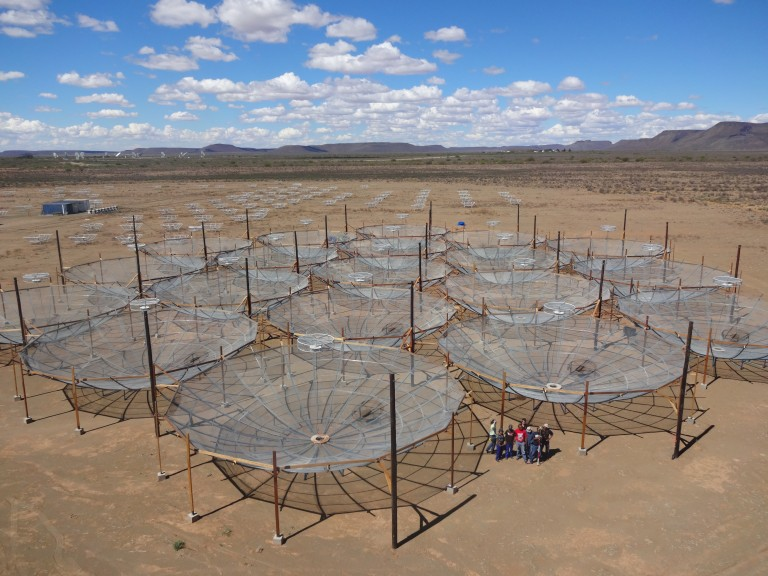
\includegraphics[width=0.85\linewidth]{figures/HERA19.png}}
\caption{HERA - Located in the Karoo desert in South Africa. The current phase of HERA consists of 37 14m parabolic dishes. In its final form, HERA will comprise 331 dishes in a closely-packed hexagonal grid. HERA is also a pathfinder project for the Square Kilometer Array (SKA).}
\end{figure}

\begin{figure}[H]
\centering
\label{fig:HERA}
\frame{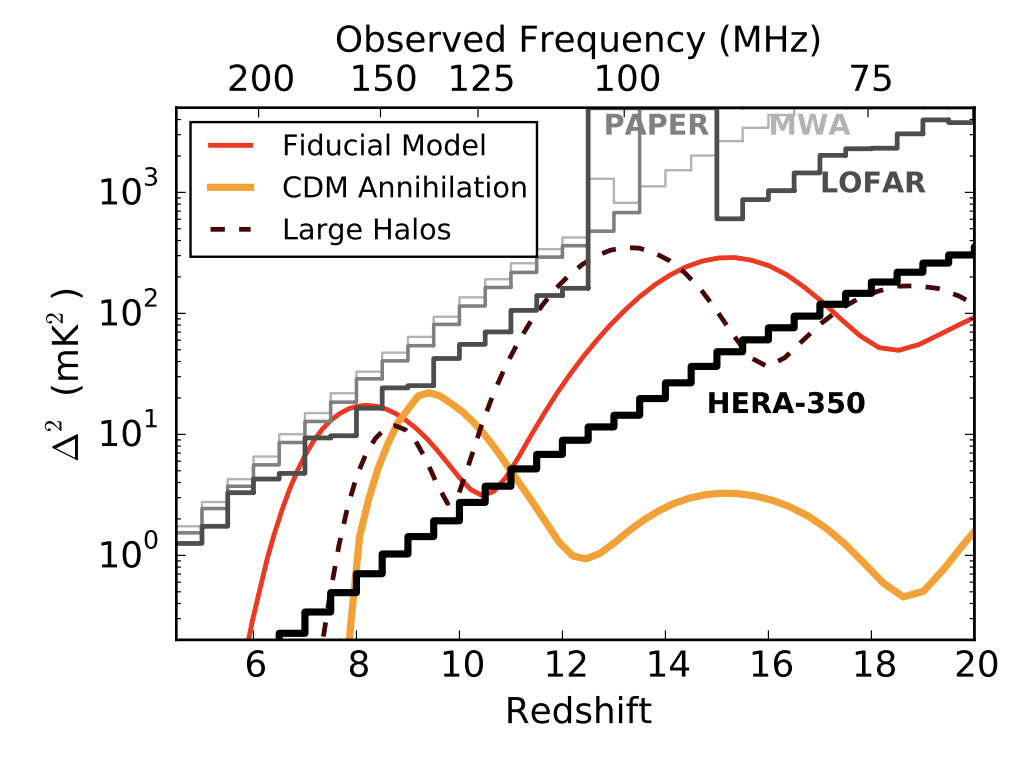
\includegraphics[width=0.9\linewidth]{figures/HERAsensitivity.png}}
\caption{Projected SNR comparison of the 350 element phase of HERA (with 1080 hrs integration time) to other low frequency arrays. Relative to several reionization models (colored), HERA-350
should have the sensitivity to measure the 21cm EoR signal across multiple redshifts.}
\end{figure}

\textbf{NOTE:}Place maybe a list or such here explaining the phased build outs and their goals. This information can be found in the HERA DeBoer 2016 paper.

%----------------------------------------------------------------------------------------
%	CONCLUSIONS
%----------------------------------------------------------------------------------------

%\color{SaddleBrown} % SaddleBrown color for the conclusions to make them stand out

%\section*{Conclusions}

%[Do we have conclusions?] [No?]


\color{DarkSlateGray} % Set the color back to DarkSlateGray for the rest of the content

%----------------------------------------------------------------------------------------
%	FORTHCOMING RESEARCH
%----------------------------------------------------------------------------------------

%\section*{Forthcoming Research}
%Probably not necessary because we can just add a blurb in the Radio Telescope arrays section about HERA?
%[Picture of HERA-331?]


 %----------------------------------------------------------------------------------------
%	REFERENCES
%----------------------------------------------------------------------------------------
% We referenced all the best people
%\nocite{*} % Print all references regardless of whether they were cited in the poster or not
%\bibliographystyle{plain} % Plain referencing style
%\bibliography{sample} % Use the example bibliography file sample.bib

%----------------------------------------------------------------------------------------
%	ACKNOWLEDGEMENTS
%----------------------------------------------------------------------------------------

%\section*{Acknowledgements}
%I refuse to acknowledge anyone or any thing!!!!!!!


%----------------------------------------------------------------------------------------
\end{multicols}
%\begin{minipage}[b]{0.19\linewidth}
%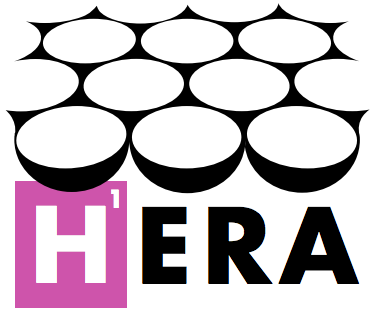
\includegraphics[width=15cm]{HERA.png} % Logo or a photo of you, adjust its dimensions here
%\end{minipage}
%\hspace{2cm}
%\begin{minipage}[b]{0.25\linewidth}
%\Huge{\textbf{PAPER}}
%\end{minipage}
%\hspace{2cm}
%\begin{minipage}[b]{0.25\linewidth}
%\Huge{\textbf{MWA}}
%\end{minipage}
\end{document}
